%pdflatex
\documentclass[13pt, letterpaper]{article}
\usepackage[utf8]{inputenc}
\usepackage[T1]{fontenc}
\usepackage[english]{babel}
\usepackage{parskip} % no indents, and nice spacing
\usepackage[margin=0.7in]{geometry} % margines

\usepackage[bitstream-charter,cal=cmcal]{mathdesign}

\usepackage{color}
\usepackage{graphicx}

\usepackage{hyperref}

\usepackage{amsmath}
\usepackage{listings} % -> also see the haskell template!
\usepackage{url}
\usepackage{xcolor}
\usepackage{microtype} % Slightly tweak font spacing for aesthetics

\usepackage{mathtools} % mathclap


\usepackage{stmaryrd} % semantics brackets \llbracket \rrbracket

\usepackage{tikz}
\usetikzlibrary{matrix}
\usetikzlibrary{positioning}
\usetikzlibrary{calc}
% \usetikzlibrary{arrows.meta}
% \usetikzlibrary{decorations.pathreplacing}
% \usetikzlibrary{fit}
% \usetikzlibrary{trees}

% pgfplots
% \usepackage{pgfplots}
% \pgfplotsset{compat=newest}

% algorithms
% \usepackage{algorithm} % the environment
% \usepackage{algpseudocode} % algorithmicx package: algorithms themselves

% "Beautiful" (i.e. sufficient) headers and footers
% \usepackage[automark,headsepline]{scrlayer-scrpage}

% \pagestyle{scrheadings}
% \clearscrheadfoot
% \automark[chapter]{section}
% \ohead{\pagemark}
% % \chead{David Mueller (\texttt{dam@jhu.edu}), On Cognition}
% \textheight=22cm

% Page number at bottom only for new chapter page
% \deftripstyle{ChapterStyle}{}{}{}{}{\pagemark}{}
% \renewcommand*{\chapterpagestyle}{ChapterStyle}

\usepackage{amsthm} % Actual theorem package.
\usepackage{thmtools} % Provides a nice frontend for (for example) amsthm.
\usepackage{centernot}
\usepackage[]{mdframed}
\usepackage[vlined,ruled]{algorithm2e}
\usepackage[most]{tcolorbox}
\tcbuselibrary{theorems}
\usepackage{cleveref}
\newtcbtheorem[no counter]
{defn}{Definition}{%                                                        
  breakable,
  fonttitle = \bfseries,
  colframe = green!30!black,
  colback = green!3
}{defn}

\newtcbtheorem[auto counter, number within = section]
{theo}{Theorem}{%                                                        
  breakable,
  fonttitle = \bfseries,
  colframe = red!55!black,
  colback = red!5
}{theo}

\newtcbtheorem[auto counter, number within = section]
{coro}{Corollary}{%                                                        
  breakable,
  fonttitle = \bfseries,
  colframe = red!55!black,
  colback = red!5
%  colframe = blue!75!black,
%  colback = blue!10
}{coro}

\newtcbtheorem[auto counter, number within = section]
{prop}{Proposition}{%                                                        
  breakable,
  fonttitle = \bfseries,
  colframe = red!55!black,
  colback = red!5
}{prop}

\crefname{defn}{definition}{Definition}
\Crefname{defn}{Definition}{Definition}

\theoremstyle{definition}
\declaretheorem[qed=$\Box$, name=Example, refname={Ex.,Exs.},numbered=no]{example}
\declaretheorem[qed=$\blacksquare$, name=Observation, refname={Obs.},numbered=no]{observation}
\declaretheorem[name=Theorem, refname={Thm.,Thms.},numbered=no]{theorem}
\declaretheorem[name=Proposition, refname={Prop.,Props.},numbered=no]{proposition}
\declaretheorem[name=Lemma, refname={Lem.,Lems.},numbered=no]{lemma}
\declaretheorem[name=Claim, refname={Cl.,Cls.},numbered=no]{claim}

% \theoremstyle{proof}
\renewcommand{\qedsymbol}{$\blacksquare$}
\newenvironment{supplementalproof}[1]{\begin{proof}[Supplemental to the proof of \cref{#1}]}{\end{proof}}

\definecolor{gray}{gray}{0.7}

\newcommand{\todo}[1]{
  {\colorbox{gray}{\begin{minipage}{\textwidth}\bfseries #1\end{minipage}}}
}

\newcommand{\inlinetodo}[1]{\textcolor{red}{#1}}

\newcommand{\new}[1]{\emph{#1}}

\newcommand{\mathtext}[1]{\;\text{#1}\;}

\renewcommand*{\mathellipsis}{%
  \mathinner{{\ldotp}{\ldotp}{\ldotp}}%
}

\newcommand{\vx}{\mathbf{x}}
\newcommand{\vr}{\mathbf{r}}
\newcommand{\bx}{\bar{\vx}}
\newcommand{\bla}{\bar{\lambda}}
\newcommand{\by}{\bar{\vy}}
\newcommand{\bz}{\bar{\vz}}
\newcommand{\vy}{\mathbf{y}}
\newcommand{\vw}{\mathbf{w}}
\newcommand{\vp}{\mathbf{p}}
\newcommand{\vq}{\mathbf{q}}
\newcommand{\vb}{\mathbf{b}}
\newcommand{\vc}{\mathbf{c}}
\newcommand{\vg}{\mathbf{g}}
\newcommand{\vd}{\mathbf{d}}
\newcommand{\vu}{\mathbf{u}}
\newcommand{\vv}{\mathbf{v}}
\newcommand{\vz}{\mathbf{z}}
\newcommand{\vlambda}{\overrightarrow{\lambda}}
\newcommand{\rarrw}{\rightarrow}
\newcommand{\vA}{A}
\newcommand{\st}{\;\; \text{s.t.} \;\;}
\newcommand{\Fg}{g_{\bar{\vx}, \vd}}
\newcommand{\vzero}{\mathbf{0}}
\newcommand{\vone}{\mathbf{1}}
\newcommand{\reals}{\mathbb{R}}
\newcommand{\notimplies}{\centernot \implies}
\newcommand{\mat}[1]{\begin{bmatrix} #1 \end{bmatrix}}
\newcommand{\dir}[2]{\frac{\delta #1}{\delta #2}}
\newcommand{\secdir}[3]{\frac{\delta^2 #1}{\delta #2 \delta #3}}

\DeclareMathOperator*{\argmax}{arg\,max}
\DeclareMathOperator*{\argmin}{arg\,min}

\newenvironment{frml}{\begin{equation*}\begin{aligned}}{\end{aligned}\end{equation*}}

% \usepackage{hyperref}
% \hypersetup{
%   pdfauthor={David Mueller},
%   pdftitle={Cognition},
%   breaklinks=true, colorlinks=false, pdfborder={0 0 0}
% }

\usepackage{enumerate}
\usepackage{float}


\title{Information Theory, Pattern Recognition, and Neural Networks}
\author{ Lecture Series by David Mackay \\ Notes by David Mueller}
\date{}
\begin{document}
\maketitle
Video series: \url{https://www.youtube.com/watch?v=BCiZc0n6COY}

\tableofcontents

\pagebreak

\section{Introduction to Information Theory}

Information theory is the study of communication over channels.
What is a channel?  Some examples of a channel are:
\begin{frml}
	Voice &\rightarrow Ears \\
	Eye &\rightarrow Brain \\
	DNA &\rightarrow DNA \\
	Antenna\;\; on\;\; Earth &\rightarrow Mars \;Rover \\
	Phone &\rightarrow Another Phone \\
\end{frml}
where the \textit{medium} of the channel is some physical system that the communication
is being transmitted over, e.g. in the case of Voice $\rightarrow $ 
Ears the medium is \textit{air}.

\begin{defn}{Fundamental Problem in Information Theory}{}
The \textbf{fundamental problem} in information theory is reliable communication 
over an unreliable channel.

\medskip
An \textbf{unreliable channel} is one where the \textit{received signal} is not equal
to the \textit{transmitted signal}, i.e.
\begin{frml}
	\text{Received Signal} \approx \text{Transmitted Signal} + \text{Noise}
\end{frml}
\end{defn}

There are two predominant soltuions that address this problem of unreliable channels.
The first option is a \textit{physical solution}, which attempts to address the physical
limitations of the medium to reduce the noise. Alternatively, there are \textit{system
solutions}, which accept the physical limitations of the channel, and attempt to
transform the overall system into a reliable one using \textit{encodings and decodings}.

Information theory is all about \textit{system solutions}. System solutions 
take the form of the pipeline below:

\begin{figure}[h!]
	\centering
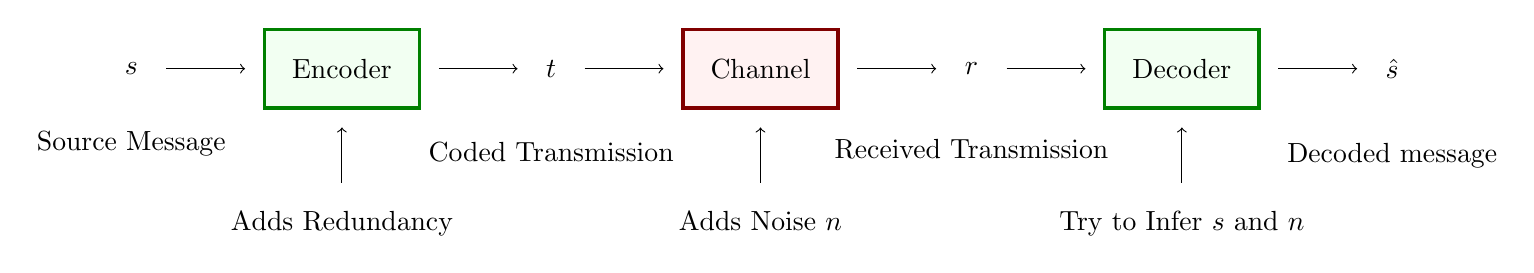
\begin{tikzpicture}
[
encdecnode/.style={rectangle, draw=green!50!black, fill=green!5, very thick, minimum size=10mm, inner sep=10},
channelnode/.style={rectangle, draw=red!50!black, fill=red!5, very thick, minimum size=10mm, inner sep=10},
every node/.style={outer sep=7}
]
%Nodes
\node[]		(1) {$s$ };
\node[]		(1t) [below=.0cm of 1] {Source Message};
\node[encdecnode]        (2)       [right=of 1] {Encoder};
\node[]		(2t) [below=.7cm of 2] {Adds Redundancy};
\node[]        (3)       [right=of 2] {$t$};
\node[]		(3t) [below=.1cm of 3] {Coded Transmission};
\node[channelnode]        (4)       [right=of 3] {Channel};
\node[]		(4t) [below=.7cm of 4] {Adds Noise $n$};
\node[]        (5)       [right=of 4] {$r$};
\node[]		(5t) [below=.1cm of 5] {Received Transmission};
\node[encdecnode]        (6)       [right=of 5] {Decoder};
\node[]		(6t) [below=.7cm of 6] {Try to Infer $s$ and $n$};
\node[]        (7)       [right=of 6] {$\hat{s}$};
\node[]		(7t) [below=.1cm of 7] {Decoded message};

%Lines
\draw[->] (1.east) -- (2.west);
\draw[->] (2.east) -- (3.west);
\draw[->] (2t.north) -- (2.south);
\draw[->] (3.east) -- (4.west);
\draw[->] (4.east) -- (5.west);
\draw[->] (4t.north) -- (4.south);
\draw[->] (5.east) -- (6.west);
\draw[->] (6.east) -- (7.west);
\draw[->] (6t.north) -- (6.south);
%\draw[->] (uppercircle.south) -- (maintopic.north);
%\draw[->] (maintopic.east) -- (rightsquare.west);
%\draw[->] (rightsquare.south) .. controls +(down:7mm) and +(right:7mm) .. (lowercircle.east);
\end{tikzpicture}
\end{figure}

In this framework, the \textit{Encoder} and \textit{Decoder} are the focus of
system solutions.

\subsection{The Binary Symmetric Channel and Disk Drives}

To examine this in more detail, let's imagine an imaginary, toy, channel.
This channel is called the \textit{Binary Symmetric Channel}.

\begin{defn}{Binary Symmetric Channel}{}
	A \textbf{Binary Symmetric Channel}, with input $x$ and output $y$, follows
	the distribution
	\begin{frml}
		&P(y = 0 | x = 0) = 1 - f \\
		&P(y = 0 | x = 1) = f \\
		&P(y = 1 | x = 1) = 1 - f \\
		&P(y = 1 | x = 0) = f \\
	\end{frml}
i.e. with probability $f$, a bit of the input $x$ will be flipped. A diagram of
this channel might look like:
	\medskip
	\begin{center}
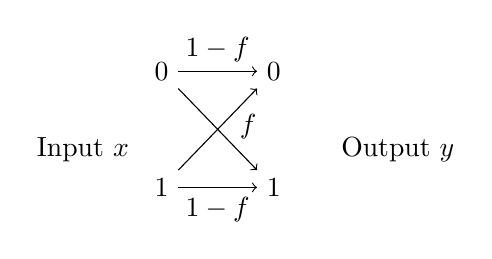
\begin{tikzpicture}
	\node[] (in) at (0,1) {Input $x$};
	\node[] (on) at (4,1) {Output $y$};
	\node[] (fn) at (2.1,1.3) {$f$};
	\node[] (tl) at (1,2) {0};
	\node[] (bl) [below=of tl] {1};
	\node[] (tr) [right=of tl] {0};
	\node[] (br) [right=of bl] {1};

	\path[->] (tl) edge node[midway, above] {$1 - f$} (tr);
	\path[->] (bl) edge node[midway, below] {$1 - f$} (br);
	\path[->] (tl) edge node[sloped, below] {} (br);
	\path[->] (bl) edge node[sloped, above] {} (tr);
\end{tikzpicture}
\end{center}
\end{defn}

Suppose we have a disk drive which follows the behavior of a binary
symmetric channel with $f = 0.1$. 

If a file of $N=10,000$ bits is stored
and then read from this disk drive, roughly how many bits will be flipped?
The answer can be modeled as a binomial distribution. 
The event of each bit being flipped or not is an independent event.
Binomial distributions have mean $Np$ and variance $Npq$, 
where in this problem $p = f$ and $q = 1 - f$.
Thus the answer is:
\begin{frml}
	\text{\# of bits flipped } = 1000 \pm 30
\end{frml}
This is \textit{not a good disk drive}. We're flipping far too many bits, here.

Instead lets ask the question: How small does $f$ need to be in order to have
a disk drive that is reliable?
Imagine that 1GB of data is written every day,
for 5 years. This results in the number of bits being sent through this
channel to be
\begin{frml}
	\text{\# of bits passed} = 5 \times 365 \times 8 \times 10^9 \approx 10^{13}
\end{frml}
In order to guarantee a 1\% chance that a any file has a single bit flipped in
5 years, then we need $f\approx10^{-15}$.
The mean and standard deviation of the number of bits flipped is modeled by
the distribution:
\begin{frml}
	\text{Mean: }&Np = 10^{13}\times10^{-15} = 10^{-2} = 0.01 \\
	\text{Std: }&\sqrt{Npq} =  \sqrt{10^{13}\times10^{-15}\times(1 - 10^{-15})} \approx 0.1
\end{frml}
Thus, with $f = 10^{-15}$ the number of bits that will flip in 5 years of use is
$0.01 \pm 0.1$

\subsection{Repitition Encoding and Decoding}

One natural way to address this problem is to add redundancy to our encoding,
increasing the chances that we can recover a source from noise.
The simplest method for adding redundancy is called the \textit{repitition code}.

\begin{defn}{Repition Code}{}
A repitition code $R_k$ encodes source $s$ by repeating each bit of $s$ $k$-times
in transmission $t$.	

\medskip
For example, $R_3$ follows the following protocol:

\medskip
\begin{center}
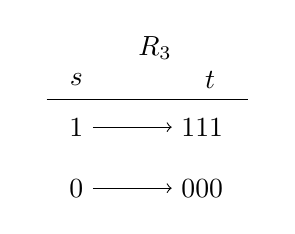
\begin{tikzpicture}
	\node[] (r) at (1.5,2) {$R_3$};
	\node[] (p1) at (0,1.35) {};
	\node[] (p2) at (2.8,1.35) {};
	\node[] (in1) at (0.5,1) {1};
	\node[] (ins) at (2.2,1.6) {$t$};
	\node[] (int) at (0.5,1.6) {$s$};
	\node[] (out1) [right=of in1] {111};
	\node[] (in0) [below=0.3cm of in1]  {0};
	\node[] (out0) [right=of in0] {000};

	\path[->] (in1) edge node[midway, above] {} (out1);
	\path[->] (in0) edge node[midway, above] {} (out0);
	\path[-] (p1) edge node[midway, above] {} (p2);
\end{tikzpicture}
\end{center}

\end{defn}

Following the $R_3$ protocol, suppose we have the following transmission:
\begin{frml}
	s &= 0 1 1 0 1 \\
	t &= 000\; 111\; 111\; 000\; 111 \\
	n &= 000\; 100\; 000\; 101\; 000 \\
	r &= 000\; 011\; 111\; 101\; 111 \\
\end{frml}

How should we decode this file? A trivial solution is to take the majority
vote of each repetition. This would recover the solution, $\hat s$ as:
\begin{frml}
	\hat s = 0 1 1 1 1
\end{frml}
Let's look at why this is the correct decoder.

\subsubsection{Decoding is Inference}

\textit{Decoding is inference}: We want to 
\textit{infer} the correct source given the recieved signal.
To do this, we need to rely on \textit{inverse probability}. 
Inverse probability relies on two fundamental rules of probability:
\begin{defn}{Fundamental Rules of Probability}{}
	There are two fundamental rules in probability.

	\medskip
The \textbf{Product Rule} states that the probability of any two random variables
is equal to the probability of one random variable times the probability of the 
other random variable given the first.
\begin{frml}
	\text{Product Rule: } P(s, r) &= P(s) P(r|s) \\
								  &= P(r) P(s|r) \\
\end{frml}

The \textbf{Sum Rule} states how to retreive a marginal probability by the
sum of all the joint variables.
\begin{frml}
	\text{Sum Rule: } P(r) &= \sum_s P(s, r)
\end{frml}
\end{defn}

Now, if we reveive an $r$, then what we want is to infer $P(s | r)$, which is
called the \textit{Posterior probability of $s$}. We can use the product rule 
combined with the sum rule to
obtain this value.

\begin{defn}{Posterior Probability of $s$ }{}
	Given a recieved signal $r$, the \textbf{posterior of $s$ } is defined as:
\begin{frml}
	P(s | r) &= \frac{P(s)P(s, r)}{P(r)} 
			 = \frac{P(s)P(s, r)}{\sum_{s'} P(r,s')}
\end{frml}
Here, we call
\begin{itemize}
	\item $P(s)$ the \textit{prior} of $s$ 
	\item $P(r,s)$ the \textit{likelihood} of $s$
\end{itemize}
\end{defn}

For example, if we are using $R_3$ over a binary symmetric channel, 
and we recieve $r = 011$, then
\begin{frml}
	P(r | s = 0) &= (1 - f) \times f \times f &= (1-f)^1 f^2\\
	P(r | s = 1) &= f \times (1 - f) \times (1 - f) &= f^1 (1 - f)^2\\
\end{frml}

If we assume that, in general,  
\begin{frml}
	P(s=0) = \frac{1}{2}, \text{ and }
	P(s=1) = \frac{1}{2}
\end{frml}
then  we can obtain the posterior distribution:
\begin{frml}
	P(s=1 | r = 011) = \frac{f(1 - f)^2\frac{1}{2}}{(1 - f)f^2\frac{1}{2} + f(1-f)^2\frac{1}{2}}
	= 1 - f
\end{frml}

Thus, given our decoding scheme for $R_3$, we can say that $P(s = 1 | r = 011) = 1 - f$, which
is $90\%$ if $f = 0.1$. So, this is a reasonable decoding scheme.
Since $P(s=1|r) > P(s=0|r)$, then $\hat s = 1$ is the best guess.

\subsubsection{Rate and Error}

Suppose we are sending a message $s$ over  Binary Symmetric Channel with flip
probability of $f$, using $R_3$ encoding and Majority Vote Decoding. 
What is the probability
that a \textit{single} bit is flipped? There are \textit{two} outcomes which must
be considered here. The probability that 3 bits in a single chunk were flipped
and the probability that 2 bits in a single chunk were flipped, i.e.
\begin{frml}
	\text{For one bit: } P(\hat s \neq s) = f^3 + 3f^2(1 - f) \approx 3f^2 - 2f^3
\end{frml}
where the $3$ comes from the $3$ different ways to \textit{choose} which bits are
flipped. This term is dominated by the $3f^2$. What have we achieved with this
encoding scheme? 
We have decreased the \textbf{rate} of our transmitting from $1$ to $1/3$. In 
doing so, we have decreased the probability of bit error from $f$ to $3f^2$.
Thus, by using 3 bits for every bit, we have achieved a \textbf{bit error rate} 
of $3f^2$.

Let's return, briefly, to the disk drive problem we were considering earlier.
Assuming again that our $f=0.1$, how many repititions do we need (i.e. what $k$ of
$R_k$) to get the bit error rate below $10^{-15}$?

It turns out that in order to achieve our desired
reliability of $10^{-15}$ 
$k$ will need to be approximately $61$. This is rather terrible, as it means
that we will need 61 \textit{individual} gigabyte disk drives in order to ensure
the reliability of a single GB disk drive.
We can do much better than this!


%\input{sections/lec02.tex}
%\input{sections/lec03.tex}
%\input{sections/lec04.tex}

\end{document}
